\section*{ROLL DECAY TEST}\label{roll-decay-test}
A common way to determine the roll damping of a ship is to conduct a
roll decay test using: model tests, CFD simulations or in some rare
cases at full scale tests. The initial heel angle during this test gives
the ship potential energy that subsequently is shifting to kinetic
energy as the ship starts to oscillate during the initial phase of the
roll decay test. The energy is transferred between kinetic and potential
energy during the oscillations. The ship loses energy over time due to
the damping as shown in Fig.\ref{fig:energy}:
\begin{figure}[H]
\begin{center}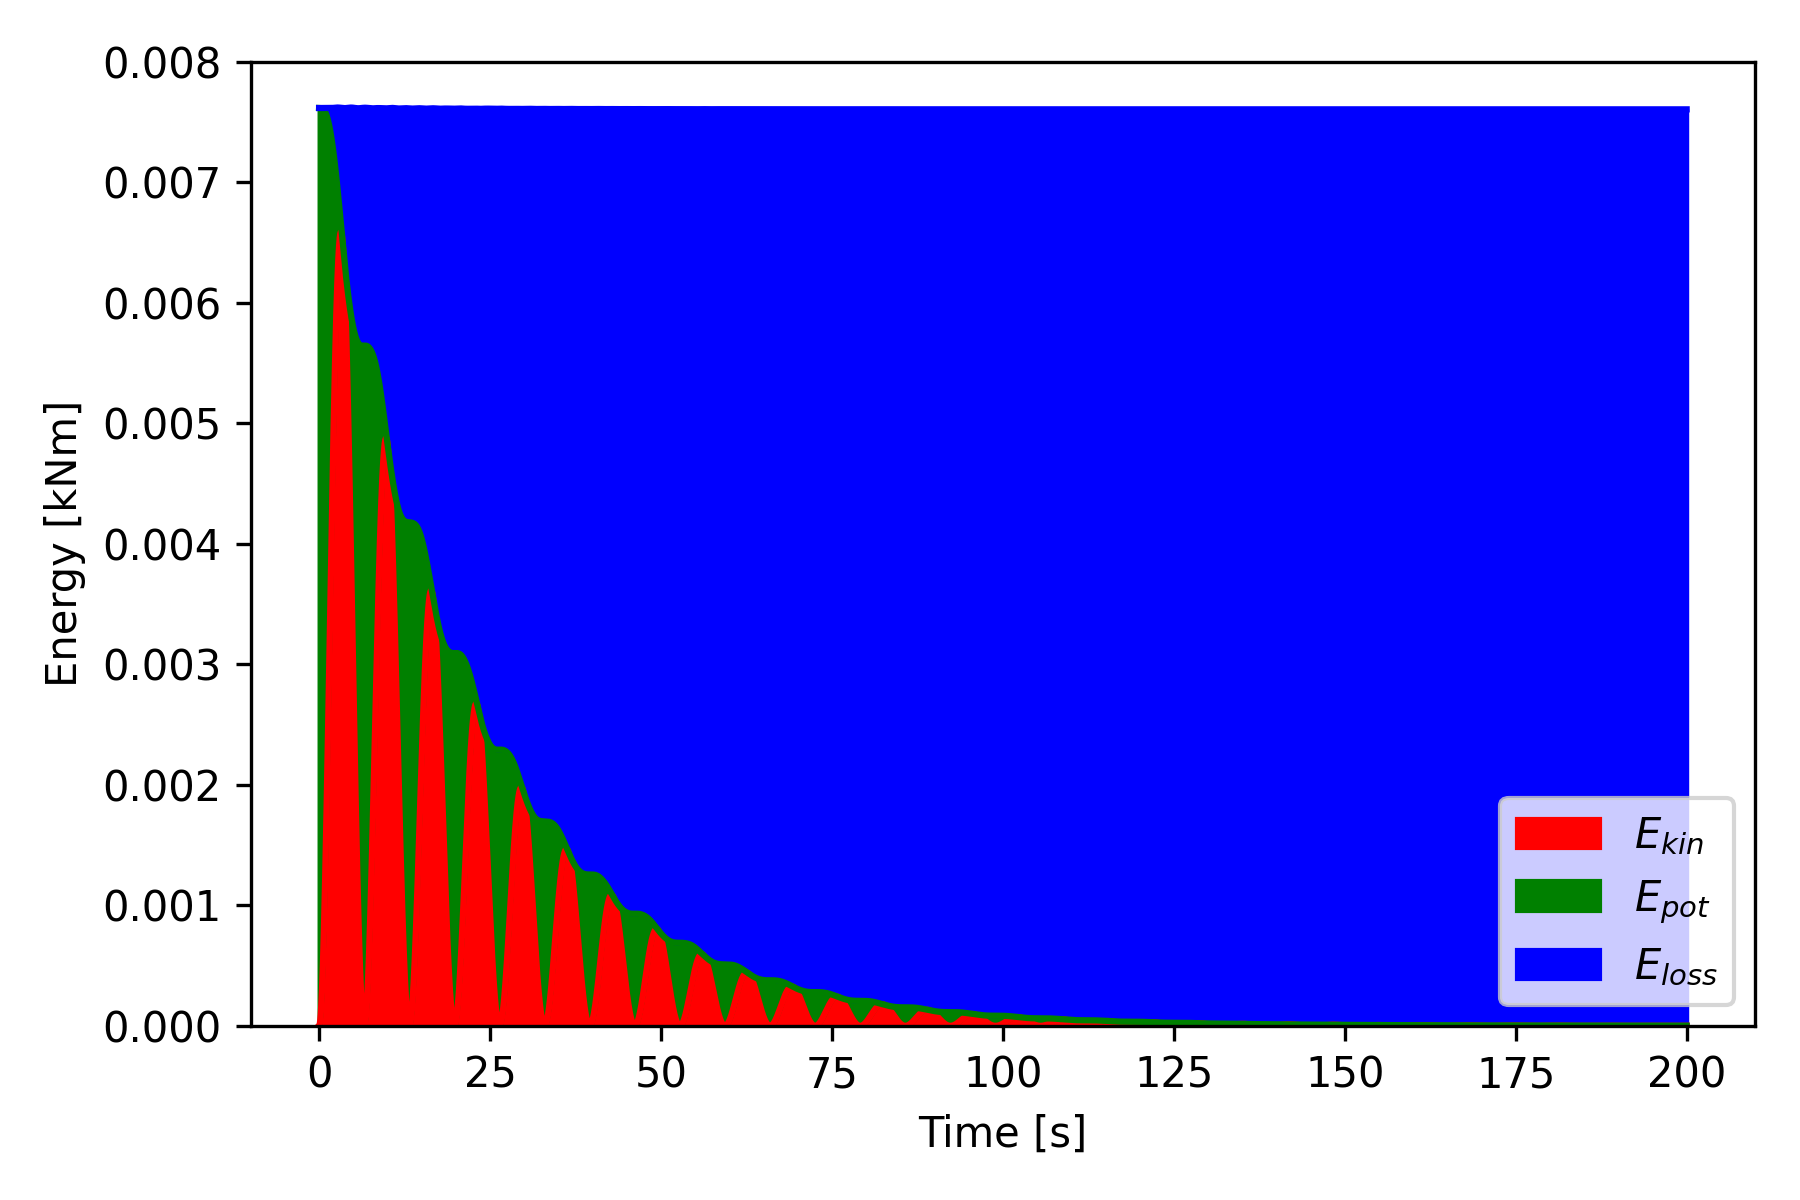
\includegraphics[width = 0.475\textwidth]{figures/energy.png}\end{center}
\vspace{-0.7cm}
\caption{Energy transfer during roll decay}
\label{fig:energy}
\end{figure}
Time traces of the roll decay, from model tests as well as from FNPF and
hybrid method simulations are used in this paper to determine the roll
damping. Two different techniques to identify the damping from these
tests are used: the PIT method, described in the next section and the
logarithmic decrement method as described in \citep{7505983/BYNJ8CFG}.
\subsection*{PIT method to estimate
damping}\label{pit-method-to-estimate-damping}
\label{se:pit}
A parameters identification technique (PIT) similar to
\citep{7505983/EXYJELCU} is used to obtain the damping coefficients from
the roll decay tests. In this technique, parameters in a mathematical
model are determined in order to get the best fit to a roll decay time
signal. A derivation of a mathematical model suitable for this study is
described below together with a description of how the parameters:
damping, stiffness and inertia coefficients are determined. The roll
decay motion can be expressed in general form according to
\citep{7505983/KL7A3RIV} which is the same equation as in
\citep{7505983/FB64RGPF} but with nonlinear stiffness:
\begin{equation}
A_{44} \ddot{\phi} + \operatorname{B_{44}}\left(\dot{\phi}\right) + \operatorname{C_{44}}\left(\phi\right) = 0
\label{eq:roll_decay_equation_general_himeno}
\end{equation}
Where $B_{44}(\dot{\phi})$ and $C_{44}(\phi)$ are the damping and
stiffness models. A quadratic model can be obtained by using cubic
damping \citep{7505983/FB64RGPF}:
\begin{equation}
\operatorname{B_{44}}\left(\dot{\phi}\right) = B_{1} \dot{\phi} + B_{2} \left|{\dot{\phi}}\right| \dot{\phi}
\label{eq:b44_quadratic_equation}
\end{equation}
And a higher order stiffness model \citep{7505983/KL7A3RIV}:
\begin{equation}
\operatorname{C_{44}}\left(\phi\right) = C_{1} \phi + C_{3} \phi^{3} + C_{5} \phi^{5}
\label{eq:restoring_equation_cubic}
\end{equation}
The total equation is then written:
\begin{equation}
A_{44} \ddot{\phi} + \left(B_{1} + B_{2} \left|{\dot{\phi}}\right|\right) \dot{\phi} + \left(C_{1} + C_{3} \phi^{2} + C_{5} \phi^{4}\right) \phi = 0
\label{eq:roll_decay_equation_quadratic}
\end{equation}
This mathematical model can be reduced to a quadratic damping model when
$B_3=0$ and a linear model when $B_2=B_3=0$. This equation does not
have one unique solution however. If all parameters would be multiplied
by a factor $k$ these parameters would also yield as a solution to the
equation. All parameters are therefore divided by the total inertia
$A_{44}$ (including added mass inertia), replacing the parameters with
new normalized parameters such as: $B_{1A} = B_1/A_{44}$. The equation
is now rewritten with these new parameters which have unique solutions:
\begin{equation}
\left(B_{1A} + B_{2A} \left|{\dot{\phi}}\right|\right) \dot{\phi} + \left(C_{1A} + C_{3A} \phi^{2} + C_{5A} \phi^{4}\right) \phi + \ddot{\phi} = 0
\label{eq:roll_decay_equation_quadratic_A}
\end{equation}
The differential equation is numerically solved as an initial value
problem, where the initial states for $\phi(t)$, $\dot{\phi}(t)$ and
$\ddot{\phi}(t)$ are used to estimate the following states, by
conducting very small time steps using the following expression for the
acceleration:
\begin{equation}
\ddot{\phi} = - B_{1A} \dot{\phi} - B_{2A} \left|{\dot{\phi}}\right| \dot{\phi} - C_{1A} \phi - C_{3A} \phi^{3} - C_{5A} \phi^{5}
\label{eq:eq_phi1d}
\end{equation}
This numerical solution can be compared with an analytical solution
\citep{7505983/KL7A3RIV} for a linear model.
For this
case the relation between nondimensional damping coefficient $\zeta$
and $B_1$ can be expressed as \citep{7505983/FB64RGPF}:
\begin{equation}
B_{1} = 2 A_{44} \omega_{0} \zeta
\label{eq:B_1_zeta_eq}
\end{equation}
and the natural frequency can be obtained from:
\begin{equation}
\omega_{0} = \sqrt{\frac{C_{1}}{A_{44}}}
\label{eq:omega0_eq}
\end{equation}
The analytical and numerical solutions are very similar according to the
example: $A_{44} = 1.0$, $B_1 = 0.3$, $C_1 = 5.0$ shown in
Fig.\ref{fig:analytical_numerical}. The numerical integration
was done with Explicit Runge-Kutta method of order 5(4) with 0.01 s time
step.
\begin{figure}[H]
\begin{center}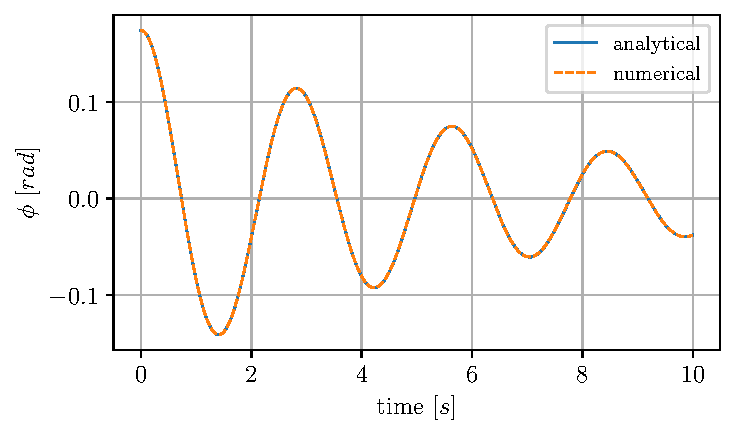
\includegraphics[width = 0.475\textwidth]{figures/analytical_numerical.pdf}\end{center}
\vspace{-0.7cm}
\caption{Comparison of analytical solution and numerical simulation of a roll decay test.}
\label{fig:analytical_numerical}
\end{figure}
The parameters of Eq.\ref{eq:eq_phi1d} can be identified using
least square fit if the time signals $\phi(t)$, $\dot{\phi}(t)$ and
$\ddot{\phi}(t)$ are all known. This is the case for the results from
the FNPF simulations but not from the model tests, where only the roll
signal $\phi(t)$ is known. The other time derivatives can be estimated
using numerical differentiation of a low-pass filtered roll signal or
Kalman filtered roll signal. The filtering will however introduce some
errors in itself. As an alternative of using this "Differentiation
approach", an "Integration approach" similar to what was used by
\citep{7505983/FJHQJJUH} and \citep{7505983/24TNAV5Z} can also be used.
The differential equation is solved numerically for estimated parameter
values determined with optimization. Gausian noise with 0.2 degrees
standard deviation was added to the simulated roll signal in
Fig.\ref{fig:analytical_numerical} to mimic measurement noise.
Fig.\ref{fig:diff_vs_int} shows a comparison between these two
approaches for a variation of the low pass filter cutoff frequency. A
very high cutoff frequency means that most frequencies pass through the
filter undisturbed. It can be seen that the estimation of damping
coefficient $B_{1A}$ with "Differentiation approach" depends very much
on the filter setting. The "Integration approach" was therefore selected
for this study, being the more accurate and robust solution. One problem
is however that the optimization needs a reasonable first guess of the
parameters to converge. The Differentiation approach was therefore used
as a pre-step to obtain a very good first guess of the parameters that
can be passed on to the Integration approach. This has been used for
both signals from FNPF and model tests, where in the latter case
numerical differentiation is used.
\begin{figure}[H]
\begin{center}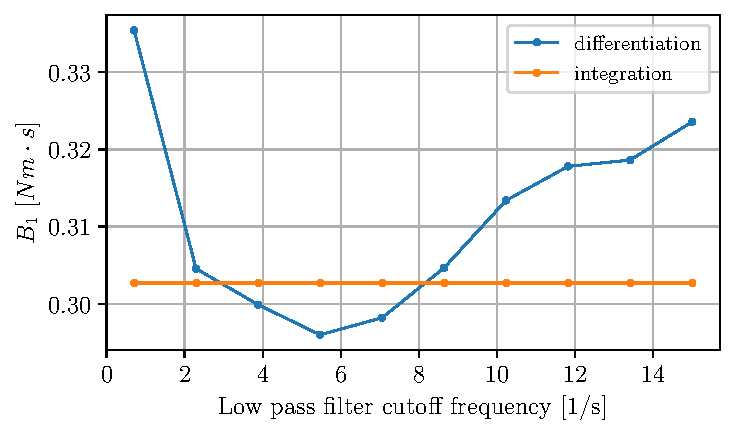
\includegraphics[width = 0.475\textwidth]{figures/diff_vs_int.pdf}\end{center}
\vspace{-0.7cm}
\caption{Comparing differentiation approach with integration approach}
\label{fig:diff_vs_int}
\end{figure}
\subsection*{Time and frequency domain}\label{time-and-frequency-domain}
\label{se:time_and_frequency} Ikeda's method is defined in the
frequency domain. The damping is expressed as function of roll angle
amplitude $\phi_a$ and roll angle frequency $\omega$. The roll decay
tests are however in the time domain, where the damping instead needs to
be expressed as function of the roll velocity $\dot{\phi}$. This can
be obtained using the equivalent linear damping $B_e$ (not to confuse
with eddy damping $B_E$). The most general way to determine $B_e$ is
to assume that the energy loss due to damping during a half cycle of
roll is the same when nonlinear and linear dampings are used
\citep{7505983/RYUBZITQ}. The $B_e$ can be calculated as a Fourier
series expansion of the damping model, which in the case of a quadratic
model yields as \citep{7505983/FB64RGPF}:
\begin{equation}
B_{e} = B_{1} + \frac{8 B_{2} \omega_{0} \phi_{a}}{3 \pi}
\label{eq:B_e_equation}
\end{equation}
$B_1$ and $B_2$ can be calculated with this equation by assuming
that the damping for a variation of roll amplitudes corresponds to the
equivalent linear damping for the same amplitudes
\citep{7505983/FB64RGPF}. This way $B_1$ and $B_2$ from the quadratic
model (Eq.\ref{eq:eq_phi1d}) fitted on roll decay tests can be
compared with corresponding values from Ikeda's method. The logaritmic
decrement method \citep{7505983/BYNJ8CFG} can be used to measure the
frequency domain quantities directly from roll decay tests (without
fitting a model first). In this method the peaks in the signal are first
measured as shown in Fig.\ref{fig:peaks}.
\begin{figure}[H]
\begin{center}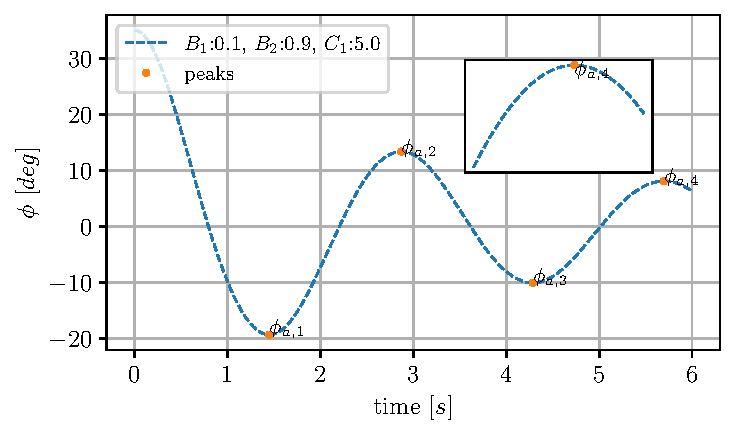
\includegraphics[width = 0.475\textwidth]{figures/peaks.pdf}\end{center}
\vspace{-0.7cm}
\caption{Analyzing peaks with logarithmic decrement method.}
\label{fig:peaks}
\end{figure}
The decrement $\Delta_n$ is calculated as the ratio between every
other peak, so that negative and positive roll peaks are separated. This
decrement can be calulated for each peak:
\begin{equation}
\Delta_n = \frac{\phi_{a,n}}{\phi_{a,n+2}}
\label{decrement}
\end{equation}
The nondimensional $\zeta$ damping coefficient for each peak can be
calculated from the logaritimic decrement \citep{7505983/BYNJ8CFG}:
\begin{equation}
\zeta_n = \frac{\delta_n}{2\pi}=\frac{ln(\Delta_n)}{2\pi}
\label{zeta_n}
\end{equation}
The dimensional damping $B_n$ (Nm*s) for each peak can be calculated
using Eq.\ref{eq:b_1_zeta_eq}.
The roll amplitude is calculated as the mean value of the three peaks in
the time window where $B_n$ is calculated:
\begin{equation}
\phi_a = (\phi_{a,n} + \phi_{a,n+1} + \phi_{a,n+2})/3
\label{phi_a}
\end{equation}
